Wolfenstein 3D is a game that needs little introduction. Released in May 1992, it achieved instant legendary status and laid down the foundations for First Person Shooter. Universaly acclaimed, the beautiful graphics, crisp digitalized sounds, engaging musics and oustanging game design made its engine sing. Within a year more than 100,000 units had been sold bringing game and a little bit of fortune to the game studio producing it: id Software.\\
\\
The many fans did not stop at completing the game. Because they wanted to modify it, they started to explore the binaries and reverse engineered them. Within a few months the assets formats were well known and people released modified version\footnote{Better know as \emph{mods}} with altered graphics, sounds effects, music and maps. The core of the game however, the secrets of its speed remained mostly unknown.\\
\\
It was closely guarded secret for an obvious reason:. A good game engine was and still is considered the main asset of a game company. As a mean to outperform competitior it is paramount to hide its algorithms and datastructures.\\
\\
But a faction within id Software did not see things that way. Instead of going along with what commercial common sense would dicate, they wanted to embrace players enthousiasm and fully open the source code to the public. After many internal struggle,[[ASK JOHN HOW HARD IT WAS.] id Software did the unthinkable: On July 21, 1995 they posted a zip archive on \emph{ftp.idsoftware.com} containing source code with instructions to build an executable.\\

 \begin{fancyquotes}
   Programming is not a zero-sum game. Teaching something to a fellow programmer doesn't take it away from you. I'm happy to share what I can, because I'm in it for the love of programming.\\
   \\
\textbf{John Carmack - Programmer}
 \end{fancyquotes}\\
\\
Pessimists would have forecasted the demise of a company foolish enough to give away its technology: Nobody had ever released the source of a mondial hit. But instead of destroying the company, it turned id Software into icon. A monument dedicated to the Right Thing that game and programmers could relate to.\\
\\
Sharing their hard gained knowledge enabled unumberable programers to become better engineers. To this day.... \\
\\
Opening the source allowed the software to live and run well after the dedicated hardware died. Twenty years after the release of Wolfenstein 3D you can still play the game on anything with a CPU and some RAM. To have the source code available had the unexpected side effect of opening a window back in time.\\
\\
As the techincal writer on \emph{fabiensanglard.net} I thought i would never take a look at this old thing that is Wolfenstein 3D code. When out of curiosity I took a peek, I could not stop reading: I was mezmerized. The more I read, the more I came to realize one very important thing: The IBM PC was designed for office work, not gaming. It was meant to crunch integers and display static images. Wolfenstein 3D made the hardware perform something it was not meant to do.\\
\\
It would be an easy mistake to look at a mips graph such as Figure \ref{fig:game_console_vs_PC} comparing the power of a PC and the gaming system of the time to conclude that because PC were so powerful it was ''easy'' to write a game for this machine. \\
\\
\begin{figure}[H]
\centering
  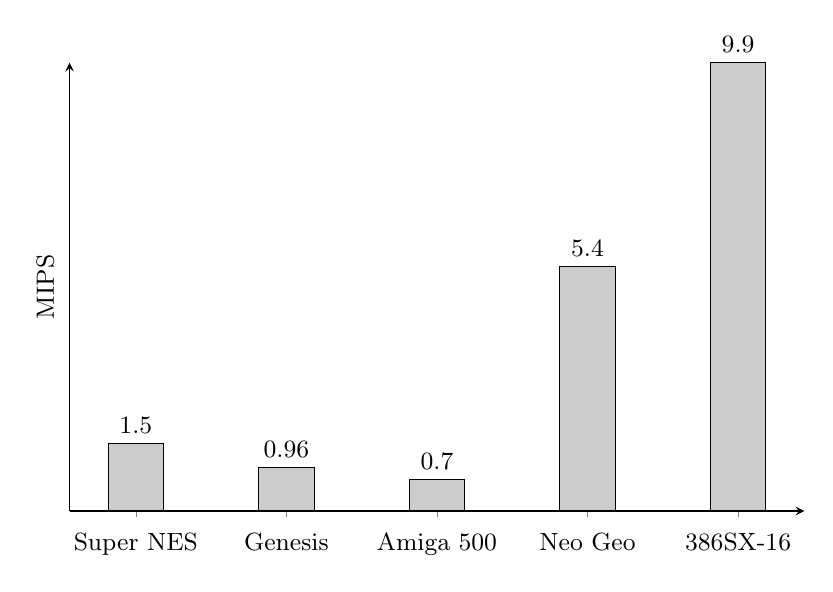
\begin{tikzpicture}[font=\small]
    \begin{axis}[
      width=0.9\textwidth,
      height=0.6\textwidth,
      ybar=6pt,
      bar width=20pt,
      ylabel={MIPS},
      ymin=0,
      ytick=\empty,
      xtick=data,
      axis x line=bottom,
      axis y line=left,
      enlarge x limits=0.11,
      symbolic x coords={Super NES,Genesis,Amiga 500,Neo Geo,386SX-16},
      xticklabel style={anchor=base,yshift=-\baselineskip},
      nodes near coords={\pgfmathprintnumber\pgfplotspointmeta}
    ]
      \addplot[fill=black!20,draw=black] coordinates {
        (Super NES,1.5)
        (Genesis,0.96)
        (Amiga 500,0.7)
        (Neo Geo,5.4)
        (386SX-16,9.9)
      };
    \end{axis}
   \end{tikzpicture}
   \caption{Game Console Vs PC.} \label{fig:game_console_vs_PC}
 \end{figure}
 
But game console were designed around animation. They all featured coprocessors and Graphic Processing Unit relying on tile engine. Animating a sprite on the screen was just about to update its $(x,y)$ coordinates.\\
\\
On the contrary, IBM PC animation was next to impossible. Not even to mention many many other obstacles. This is where the root of my admiration for Wolfenstein 3D started: id Software achieved the impossible by building a game engine able to not only workaround the many limitations of the machine but sometimes turn them into an advantage.\\
\\
I see beauty in the ability to repurpose a machine to do something even the builder did not think was possible. It takes optimist, creativity, passion and dedication to be able to leave the safe harbour of ''intended design'' in order to Explore, Dream and Discover. This is what this book is dedicated to.\\
\bigskip

 \textbf{\underline{Disclaimer :}} The description that follows is very technical and will appeal mostly to programmers. If you are more into the human aspect of game programming I would recommend instead to read David Kushner’s chef d’oeuvre: “Masters of Doom: How Two Guys Created an Empire and Transformed Pop Culture”.
This book tries to give a detailed story of how Wolfenstein 3D was done. It is divided in three parts reviewing the hardware, the team and the software.